\section{Magnetization per Spin}\label{sec:res:magnet}
	\subsection{Observable}\label{sec:res:magnet:observable}
		\Observable{Metropolis}{Magnetization}{magnetization}
		\Observable{Wolff}{Magnetization}{magnetization}
		Studying the total absolute magnetization per spin for the Metropolis (\cref{fig:obs:Metropolis:Magnetization}) and Wolff (\cref{fig:obs:Wolff:Magnetization}) algorithms shows that, for low temperatures, the magnetization tends to $1$, indicating the existence of a quasi-ordered low-temperature state. With increasing temperature, the magnetization decreases steadily at first and then rapidly until it slowly levels out in the unordered high-temperature state. One can also see finite-size effects as, for increasing lattice sizes, the form of the curve becomes more pronounced. The curve generally levels out to $0$, which cannot be observed for small lattice sizes in our temperature interval. The errors can be found in~\Cref{sec:errors:magnetization} of~\Cref{chap:errors}.
		
		\paragraph{Magnetization Squared per Spin}\label{sec:res:magnetsquare} The plots for the absolute total magnetization per spin, its autocorrelation function, and integrated autocorrelation time can be found in~\Cref{sec:observables:magnetization_squared}, and the errors can be found in~\Cref{sec:errors:magnetizationsquare} of~\Cref{chap:errors}.
	
	\subsection{Magnetic Susceptibility per Spin}\label{sec:res:xs}
		\Observable{Metropolis}{MagneticSusceptibility}{magnetic susceptibility}
		\Observable{Wolff}{MagneticSusceptibility}{magnetic susceptibility}
		The magnetic susceptibility $\chi$ can be derived from $\langle M \rangle$ and $\langle M^2 \rangle$ according to~\Cref{eq:magnetic_suceptibility}.  Comparing the curve of the Metropolis (\cref{fig:obs:Metropolis:MagneticSusceptibility}) and Wolff (\cref{fig:obs:Wolff:MagneticSusceptibility}) algorithms reveals a similar form. The magnetic susceptibility is decreasing for low and high temperatures. A peak exists near the critical temperature, which slowly shifts to the left and becomes narrower as the lattice size increases and the peaks' magnitude decreases. The errors can be found in~\Cref{sec:errors:magneticsusceptibility} of~\Cref{chap:errors}.
		
		When zooming in on the $\chi$ peak for the Metropolis (\cref{fig:obs:Metropolis:MagneticSusceptibilityZoom}) and Wolff (\cref{fig:obs:Wolff:MagneticSusceptibilityZoom}) algorithms, we see that near criticality, the curve of $X$ obtained using the Wolff algorithm is substantially smoother. The data points follow a very predictable trajectory,  which gives us the confidence that if we were to increase the temperature scanning depth to $\geq 3$, we would not zoom in on the wrong neighbourhood.
		\Observable{Metropolis}{MagneticSusceptibilityZoom}{zoomed-in magnetic susceptibility}
		\Observable{Wolff}{MagneticSusceptibilityZoom}{zoomed-in magnetic susceptibility}
	
	\subsection{Estimating \texorpdfstring{$T_C$}{T} using the Magnetic Susceptibility \texorpdfstring{$\chi$}{X}}\label{sec:res:temperature}
		As shown by~\citet[eq. 3]{shifted}, there exists a shifted temperature $T^*$ that asymptotically approaches the critical temperature $T_C$ for an infinite lattice
		\begin{equation}\label{eq:shifted_temperature}
			T^*(L) \approx T_C + \frac{\pi^2}{4c (\ln{L})^2}.
		\end{equation}
		The shifted temperature gives us a way to estimate the critical temperature $T_C$. We take the maximum magnetic susceptibility $\chi_\text{max}$ per lattice size from~\Cref{fig:obs:Metropolis:MagneticSusceptibility} and, in~\Cref{fig:critical_temperature}, plot the temperature $T$ where it occurs against $(\ln{L})^{-2}$. The errors are taken from the distance between two data points, as the peak could be slightly left or right of $\chi_\text{max}$.
		\begin{figure}[htbp]
			\centering
			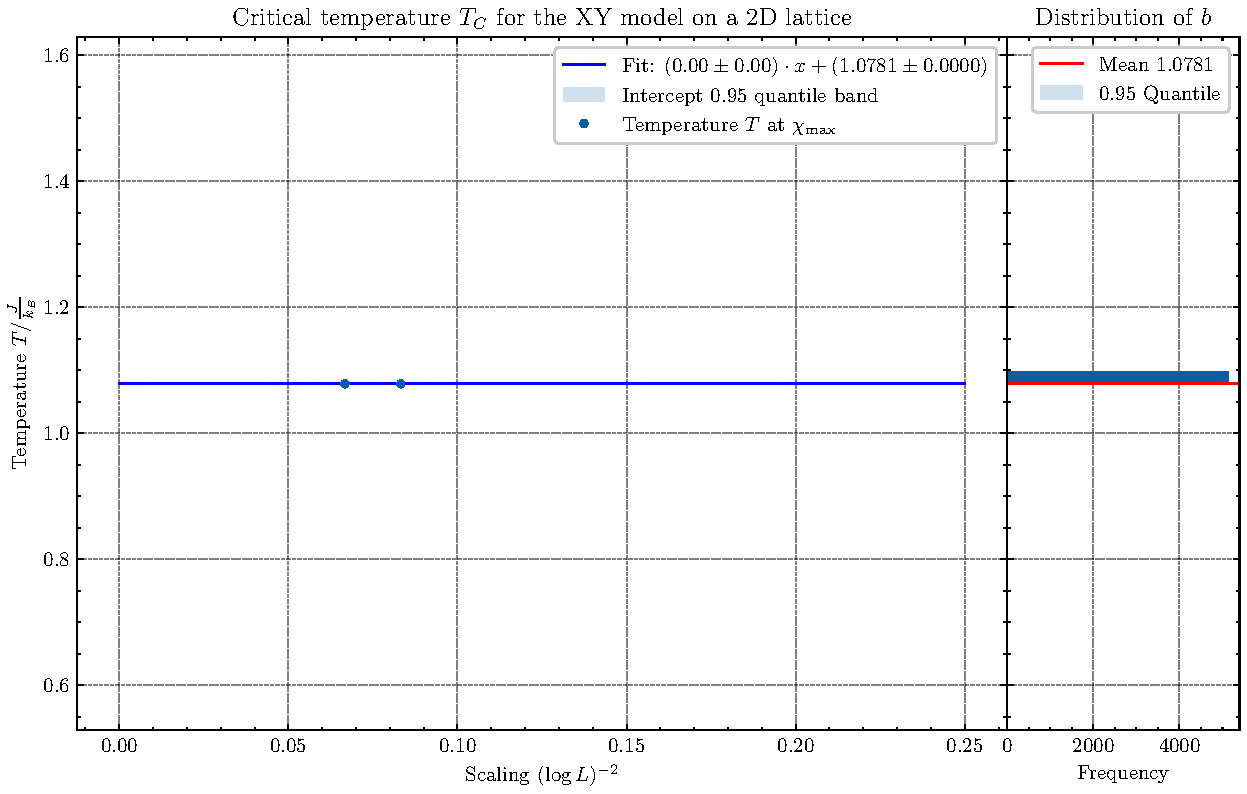
\includegraphics[width=0.8\textwidth]{../figures/Metropolis/Critical_Temperature.pdf}
			\caption[Estimating $T_C$ using the Metropolis algorithm by plotting $T$ where $\chi$ is maximal against $(\ln L)^{-2}$]{The temperature at which $\chi$ is maximal against $(\ln L)^{-2}$ yields a linear correlation and confirms~\Cref{eq:shifted_temperature} for the Metropolis algorithm.}
			\label{fig:critical_temperature}
		\end{figure}
		
		We fit a linear regression model using \emph{SciPy's ODR}\footnote{\url{https://docs.scipy.org/doc/scipy/reference/odr.html\#introduction}} method against our data points, which confirms the correlation of lattice size and shifted temperature. The intercept of the fit gives the estimate for the critical temperature. To estimate our errors, we used a bootstrap approach by resampling $\num{10 000}$ times from our measurements and redoing our linear regression model each time. The standard deviation $\sigma$ of our bootstrapped intercepts was taken as the error of our $T_C$ estimate. For the Metropolis algorithm, we estimate:
		\begin{equation}
			T_{C, \text{Metropolis}} = \SI{0.8902(118)}{\J\per\kb}.
		\end{equation}
		
		For the Wolff algorithm, we can, thanks to the smoother $\chi$ curve (\cref{fig:obs:Wolff:MagneticSusceptibilityZoom}), go one step further and account for the choice of $L$. The expectation is that the $T_C$ estimate becomes more accurate when we do not account for small lattice sizes and $L \rightarrow \infty$. We iteratively do the same procedure, as we did for the Metropolis algorithm, now for the Wolff algorithm, while taking away the next smallest lattice size on each iteration. The smallest lattice size still used is our cutoff lattice size $L_\text{min}$, which we increase until $L_\text{min} = 256$, as we still need enough data points to perform our linear regression and bootstrapping procedure.
		
		\begin{figure}[htbp]
			\centering
			\includegraphics[width=0.8\textwidth]{../figures/Wolff/Critical_Temperature_Scaling.pdf}
			\caption[Estimating $T_C$ by accounting for the cutoff lattice sizes $L_\text{min}$]{The critical temperature estimate $T_C$ dependence on the lattice cutoff size $L_\text{min}$ for $L_\text{min} = \{4, \dots, 256\}$ for the Wolff algorithm}
			\label{fig:critical_temperature_scaling}
		\end{figure}
		\begin{figure}[htbp]
			\centering
			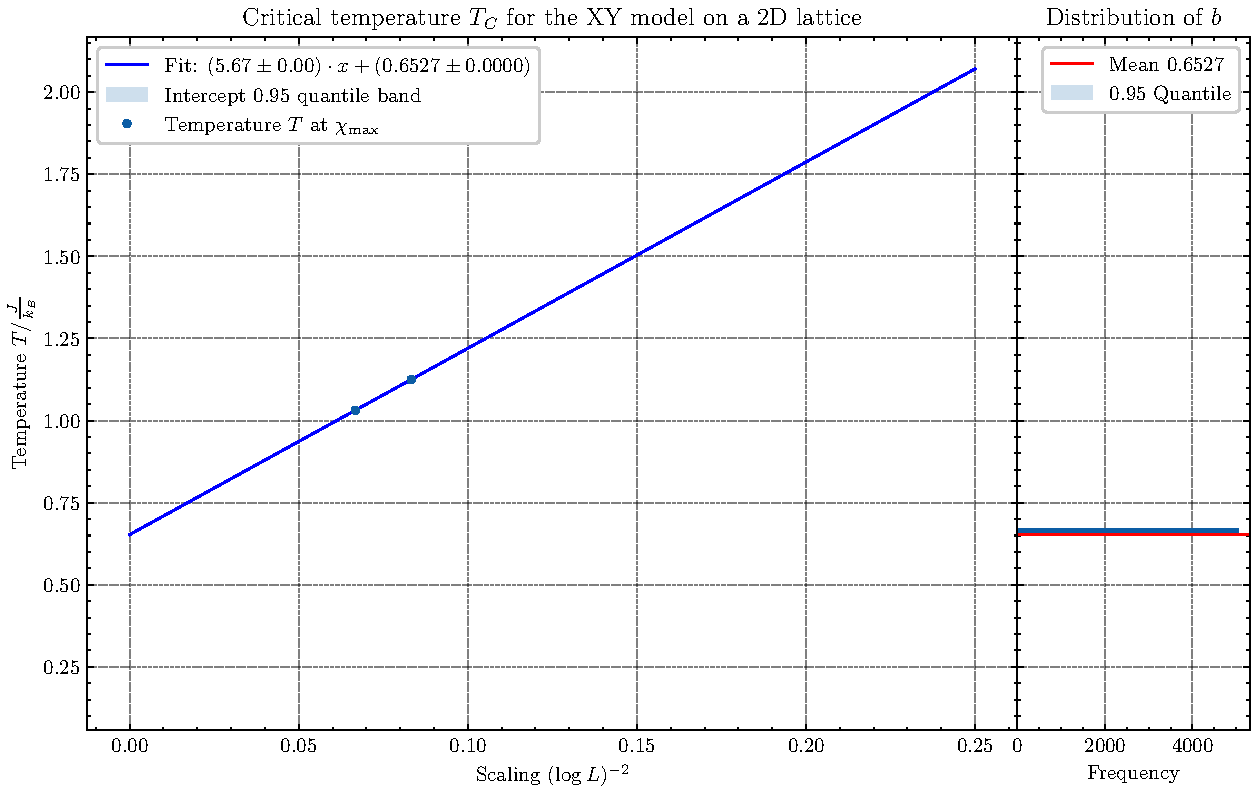
\includegraphics[width=0.8\textwidth]{../figures/Wolff/Critical_Temperature.pdf}
			\caption[Estimating $T_C$ by extrapolating the lattice size $L \rightarrow \infty$]{Estimating the critical temperature $T_C$ by extrapolating the lattice sizes $L \rightarrow \infty$ and simultaneously omitting smaller lattice sizes for the Wolff algorithm.}
			\label{fig:critical_temperature:wolff}
		\end{figure}
		
		In~\Cref{fig:critical_temperature_scaling}, we plotted the resulting $T_C$ estimates against the cutoff lattice size $L_\text{min}$. We observe that for an increasing cutoff, the $T_C$ estimate approaches a fixed value. The errors are larger for small cutoffs because we cannot accurately determine $\chi_\text{max}$, as well as for bigger cutoffs, as we have fewer data points to sample from. The plot indicates that the estimate for $T_C$ scales with $L_\text{min}^{-1}$. In~\Cref{fig:critical_temperature:wolff}, we therefore plot $T_C$ against $L_\text{min}^{-1}$ and bootstrap the data points using the same procedure as before. Our final estimate for the $T_C$ is given by the intercept of our fit:
		\begin{equation}
			T_{C,~\text{Wolff}} = \SI{0.8934(9)}{\J\per\kb}.
		\end{equation}
		This value represents the estimated $T_C$ if we were to simulate bigger and bigger lattice sizes while simultaneously starting to omit smaller ones.
		
		We can compare our results $T_{C,~\text{Metropolis}} = \SI{0.8902(118)}{\J\per\kb}$ and $T_{C,~\text{Wolff}} = \SI{0.8934(9)}{\J\per\kb}$ with some literature values:
		\begin{itemize}
			\item In~\citet{literature_gpu}, the authors used a GPU-based Monte Carlo approach to estimate the critical temperature to $T_C=\SI{0.8935(1)}{\J\per\kb}$.
			\item In~\citet{literature_cpu}, the authors used a CPU-based Monte Carlo approach to estimate the critical temperature to $T_C=\SI{0.89213(10)}{\J\per\kb}$.
			\item A theoretical transfer matrix approach employed by~\cite{literature_theo} led to a critical temperature of $T_C \approx \SI{0.8916}{\J\per\kb}$.
		\end{itemize}
		
		The literature values are compatible with our estimated $T_{C,~\text{Metropolis}}$. which indicates that our implementation is correct and our temperature \emph{zoom} procedure works. The errors, however, are quite large, and the compatibility of our estimate might just be because of that. We are approaching the limits of what can be done with the Metropolis algorithm given our time and resource constraints. At big lattice sizes, the $\chi$ estimates (\cref{fig:obs:Metropolis:MagneticSusceptibilityZoom}) are not accurate enough to determine $\chi_\text{max}$. 
		
		For the Wolff algorithm, our estimate is in very good agreement with the literature values. The reduced effects of critical slowing-down are clearly visible, and our procedure to account for the choice of $L$ yields good results. The error is smaller by a factor of $\approx 10$ compared to our Metropolis estimate, which is another indicator of the advantages of the Wolff algorithm.
